\documentclass[a4paper]{article}

\usepackage[english]{babel}
\usepackage[utf8]{inputenc}
\usepackage{amsmath}
\usepackage{amssymb}
\usepackage{float}
\usepackage{graphicx}
\usepackage[colorinlistoftodos]{todonotes}
\usepackage[authoryear]{natbib}
\usepackage{hyperref}
\usepackage{authblk}
\usepackage{fancyhdr}
\usepackage[margin=1in]{geometry}
\usepackage{pgfplots}
\usepackage{parskip}
\usepackage{graphicx}
\pgfplotsset{compat=1.12}

\usepackage{datetime2}

\title{Automated Planning - Lab 6}
\author{Victor Tranell Erik Linder-Norén}
\date{\today}

\begin{document}

\maketitle
In this report the following two environments and robots will be used:
\begin{itemize}
    \item Environment 1: Maze, robot: hook\_planar\_robot.dae
    \item Environment 2: Barriers, robot: barriers\_easy\_robot.dae
\end{itemize}

\section*{Planner 1: PRM}
This is a probibalistic planner that randomizes states along the availible state space. Creates roadmaps around milestones which leads to a high granularity map along obstacles.

\textbf{Observations:}
Since it explores around obstacles the path will be very good around them. However, not all obstacles must be avoided since they are not along the best paths and therefore PRM does not compute the best paths and is generally pretty slow.

\begin{figure}[H]
     \centering
     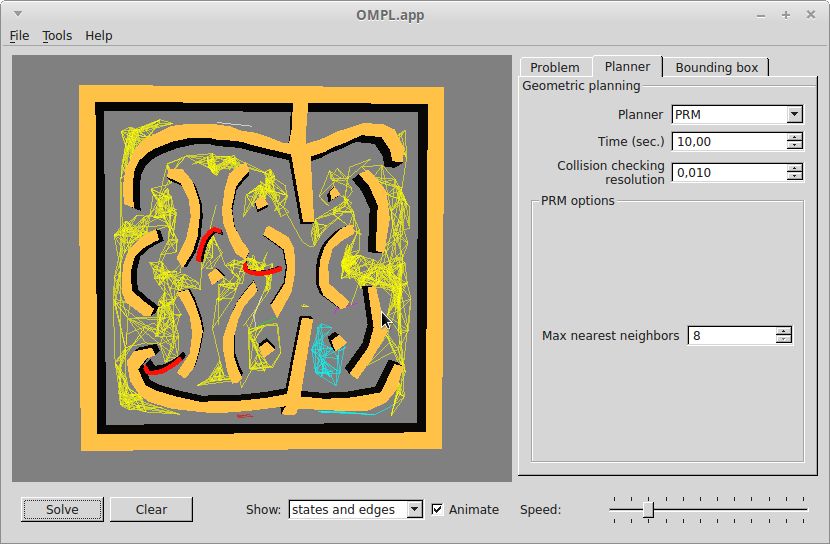
\includegraphics[width=0.6\textwidth]{prm_maze.png}
     \caption{PRM, Maze}
     \label{signals}
\end{figure}

\begin{figure}[H]
     \centering
     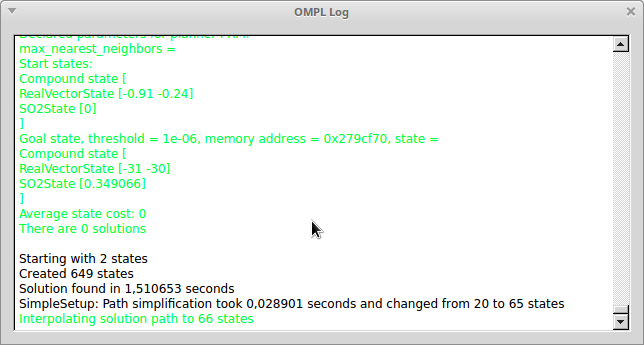
\includegraphics[width=0.6\textwidth]{prm_maze_log.png}
     \caption{PRM, Maze log file}
     \label{signals}
\end{figure}

\begin{figure}[H]
     \centering
     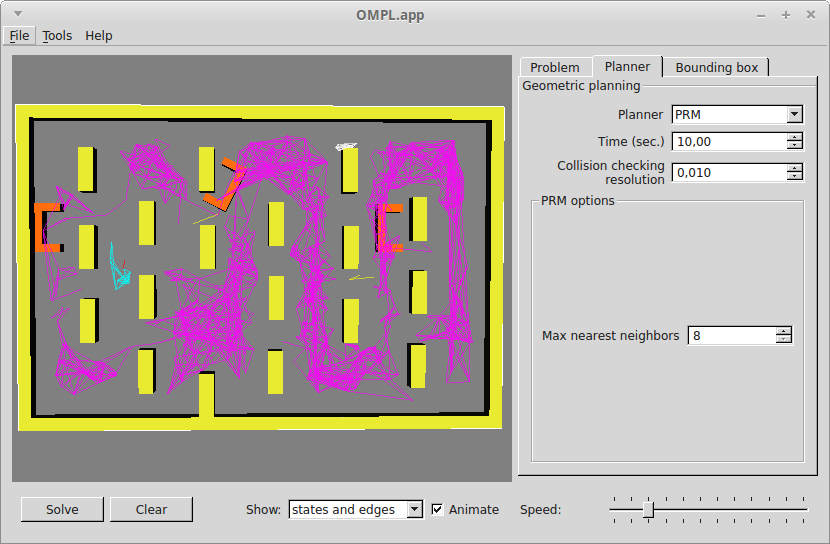
\includegraphics[width=0.6\textwidth]{prm_barrier.png}
     \caption{PRM, Barriers}
     \label{signals}
\end{figure}

\begin{figure}[H]
     \centering
     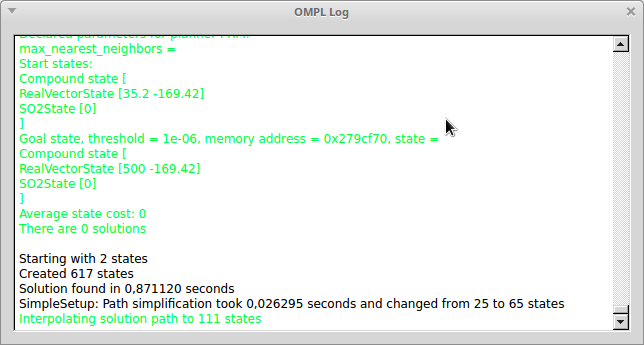
\includegraphics[width=0.6\textwidth]{prm_barrier_log.png}
     \caption{PRM, Barriers log file}
     \label{signals}
\end{figure}

\section*{Planner 2: RRTConnect}
RRTConnect uses two RRT searches, one from the start position and one from the goal and tries to connect them. An RRT search is performed by randomly placing state on the map and then connects it to the closest state already explored until the goal state is found. 

\textbf{Observations:}
This is generally very quick and finds good solutions. This is due to the fact that it starts both from the goal and start state and only expands states that are closer to the current node than any previously explored state.

\begin{figure}[H]
     \centering
     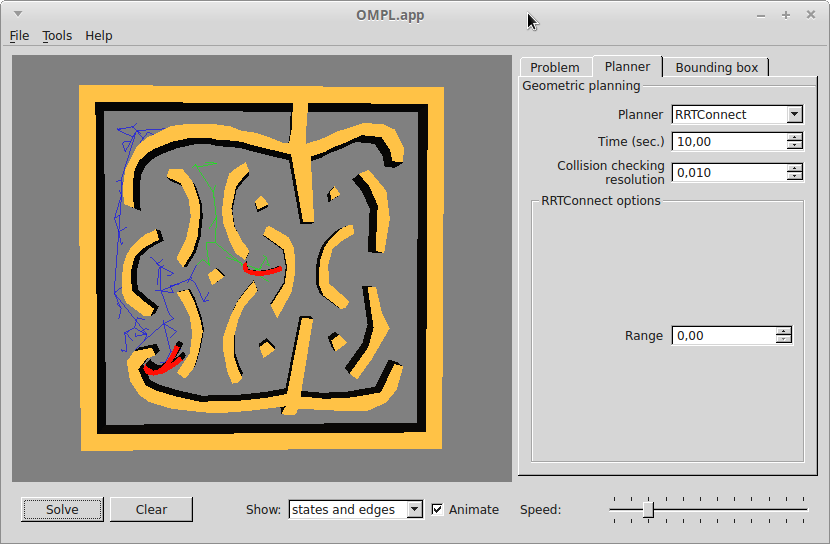
\includegraphics[width=0.6\textwidth]{rrtconnect_maze.png}
     \caption{RRTConnect, Maze}
     \label{signals}
\end{figure}

\begin{figure}[H]
     \centering
     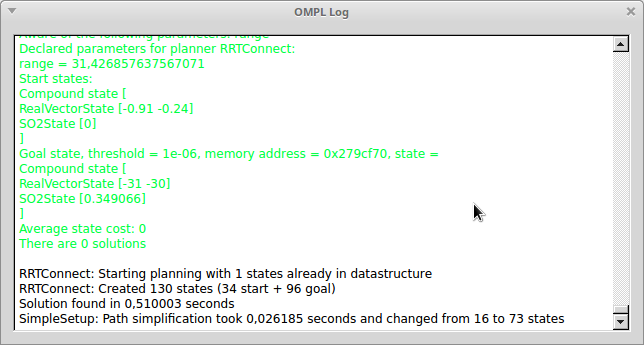
\includegraphics[width=0.6\textwidth]{rrtconnect_maze_log.png}
     \caption{RRTConnect, Maze log file}
     \label{signals}
\end{figure}

\begin{figure}[H]
     \centering
     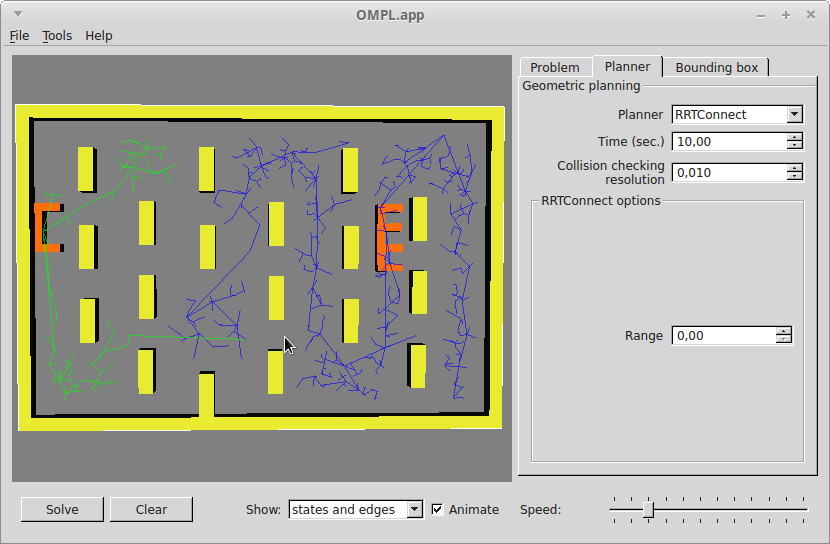
\includegraphics[width=0.6\textwidth]{rrtconnect_barrier.png}
     \caption{RRTConnect, Barriers}
     \label{signals}
\end{figure}

\begin{figure}[H]
     \centering
     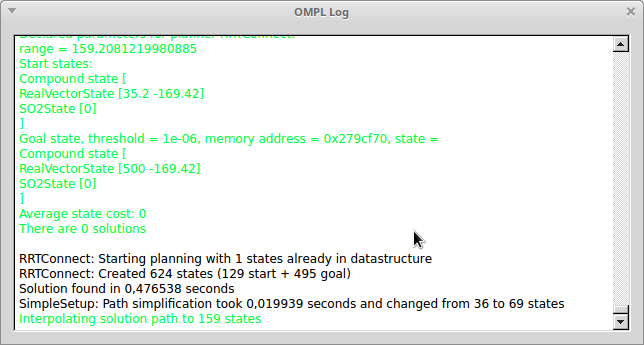
\includegraphics[width=0.6\textwidth]{rrtconnect_barrier_log.png}
     \caption{RRTConnect, Barriers log file}
     \label{signals}
\end{figure}

\section*{Planner 3: SPARStwo}
Places randomly uniformly distributed states among the entire search space and tries to connect it between each other to generate a roadmap. Since it doesn't consider distance between the connected states it is not very reliable in finding good paths. Since the points are so sparsly distributed it only considers a small amount of states.

Env1.
This is very similar to the PRM in the same environment since the PRM expands around obstacles and the whole map consist of obstacles and therefore sparstwo and PRM has similarly sized search spaces. However it is far from optimal.

Env2.
Since this map is very big the availible search space is huge which leads to it taking a long time as sparsetwo selects randomly over the whole map. However it is far from optimal.

\begin{figure}[H]
     \centering
     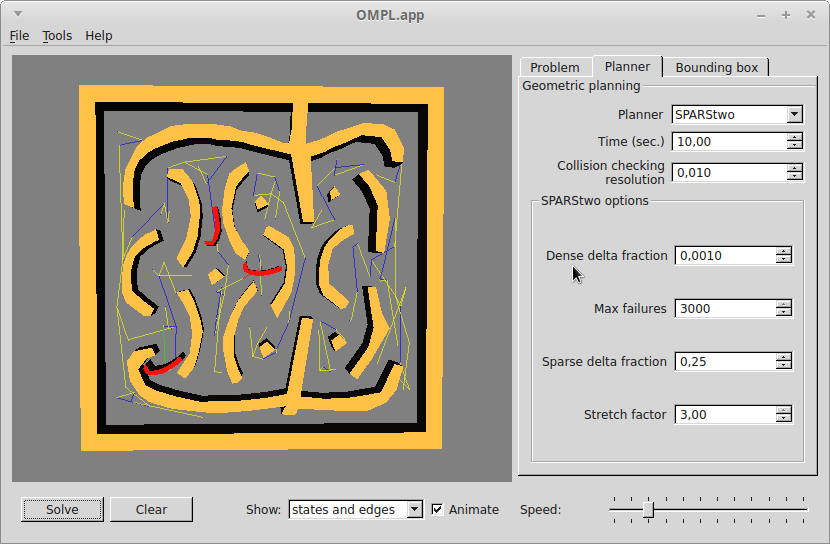
\includegraphics[width=0.6\textwidth]{sparsetwo_maze.png}
     \caption{SPARStwo, Maze}
     \label{signals}
\end{figure}

\begin{figure}[H]
     \centering
     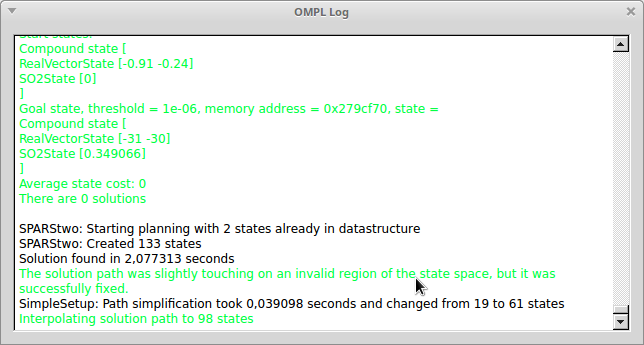
\includegraphics[width=0.6\textwidth]{sparsetwo_maze_log.png}
     \caption{SPARStwo, Maze log file}
     \label{signals}
\end{figure}

\begin{figure}[H]
     \centering
     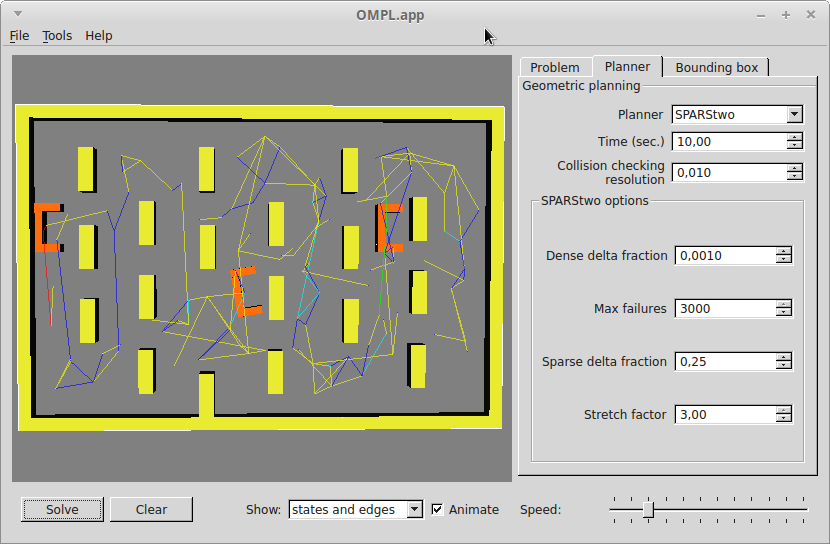
\includegraphics[width=0.6\textwidth]{sparstwo_barrier.png}
     \caption{SPARStwo, Barriers}
     \label{signals}
\end{figure}

\begin{figure}[H]
     \centering
     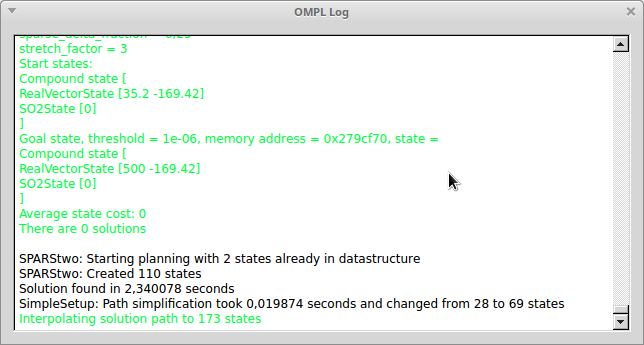
\includegraphics[width=0.6\textwidth]{sparsetwo_barrier_log.png}
     \caption{SPARStwo, Barriers log file}
     \label{signals}
\end{figure}

\end{document}